\chapter{Routing agent policy design}
\label{chapter:learning}

 \section{Introduction}
In this chapter we describe basic policies used in previous work and their shortcomings, the policies that we have implemented and their benefits. We also discuss how these policies were designed and structure of learning used to achieve the best results.

\section{Environment interface}
The general interface between agent and environment for this problem has already been described in chapter~\ref{chapter:problem}. However, it left out one important detail. When using the softmin routing strategy, one of the parameters for input to the softmin function was a value $\gamma$. In their paper, Valadarsky et al.\cite{valadarsky2017learning} set this value to $2.0$. They also only ran their experiments on a single graph. We quickly realised that the best value to use for $\gamma$ would also depend on the topology of the graph used, and so although it was a hyperparameter in prior work, now that the graph changing is part of the problem space, $\gamma$ also has to be output from our agent and so it placed into the action space.

\section{Standard policies}
We use two policies as baselines to compare the new GNN-based method against. The first of these is a multilayer perceptron (MLP)\cite{rumelhart1986learning}. In this case we use a fully-connected network as that is the kind used in previous work. It is important to note that this policy does not take into account any of the structure of the problem so it is in effect the simplest approach. However, it is also the least flexible as its input and output sizes are both fixed. This means that it can only be trained and used on one graph and with one length of history for the observations to be passed in.

We then extend this model to use an LSTM\cite{hochreiter1997long}. This is because the history structure of the observations is limiting and only works if we know it is longer than any regularity we wish to find, The LSTM model is different in that at each timestep the observation that it receives is only the previous DM with the hope that it will learn to interpret the history in some meaningful way using its memory. This is beneficial as it allows for flexibility of history length and means that less structure in the problem is assumed. However, it still suffers from the same issue that the MLP does. Namely that it has a fixed size input and output meaning that it can only be trained and used on a single graph. In fact it is potentially possible to use an LSTM in a similar way to the iterative GNN model described in section~\ref{section:gnn_iterative} but that is beyond the scope of this research. A diagram of the MLP and LSTM policies can be seen in figure~\ref{fig:mlp_lstm}.

\begin{figure}
    \centering
    
\includegraphics[width=0.8\textwidth]{figures/mlp_lstm.pdf}
    \caption{The structure of the MLP and LSTM policies for data-driven routing. On the left is a representation of the MLP policy and on the right is a representation of the LSTM policy.}
    \label{fig:mlp_lstm}
\end{figure}


\section{GNN policy}
\label{section:gnn_policy}
The new work is introduced here with the application of GNNs to the problem. The first stage of this was to make sure that a GNN can perform routing as well as the MLP can. This meant that we started off with the constricted space where we read out an entire routing from the GNN policy as a single action. Due to the nature of training frameworks this unfortunately allows us to only train the network on one graph as the output size must be fixed and is the number of edges of the graph. However, does allow us to apply the trained model to different graphs.

When deciding what form the GNN should take there are in fact many different types to choose from. For example, there is the graph attention network (GAT)\cite{velivckovic2017graph} which uses self-attention when propagating and is parallelisable, and message-passing neural networks (MPNNs)\cite{gilmer2017neural} which first generalised different types of GNN that pass data along edges and combine it in some way. In this specific problem we need outputs on edges and inputs on nodes so it is important that the model derives edge features taking into account node features. It is also the case that the amount of demand to and from a specific node can have a global impact as it is possible that such a flow will be destined for the most distant vertex from this one. Therefore, the structure will have to be able to take into account global information when setting edge weights. Finally, the structure of the graph in the way its edges connect has a large impact on how flows can be routed and their resulting impact on utilisation. To properly take advantage of this, our policy must be able to see how information flows and so must make use of the edges. Given these requirements it makes sense to use the one of the most general kinds of GNN so as not to place accidental restrictions on learning.

In keeping with the above observations, we settled on using a fully connected graph network block as defined by Battaglia et al.\cite{battaglia2018relational} and shown in section~\ref{section:graph_neural_networks} as this is the most general method achievable with the framework and means that we have not constricted any information flows unnecessarily. We also are aware that constricting the feature vectors for edges and vertices to length one and two respectively due to the input and output sizes may make learning less efficient and results worse. Therefore, we expand from the core processing GN block to an encode-process-decode model. This consists of first mapping all the node features using a learned function to larger hidden size, then performing some number of computation steps by the core network and finally mapping all of the edge features to the correct output size using another learned function. The structure of this policy can be seen in figure~\ref{fig:encode_process_decode}.

\begin{figure}
    \centering
    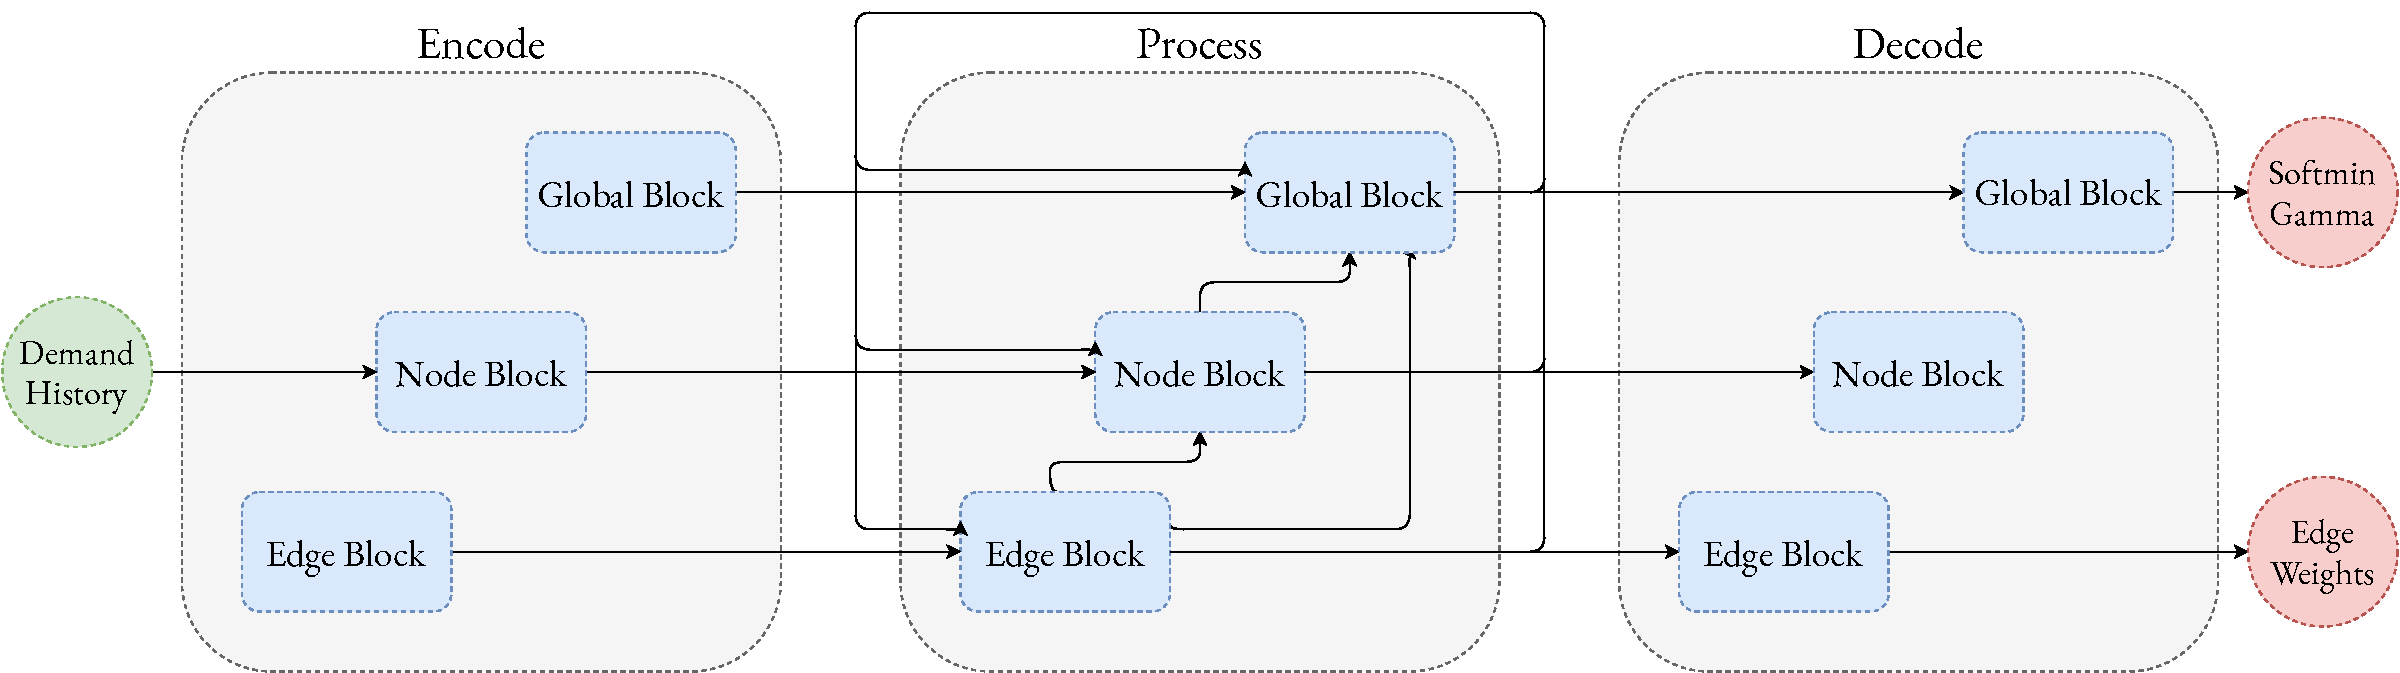
\includegraphics[width=\textwidth]{figures/encode_process_decode.pdf}
    \caption{The encode-process-decode GNN structure. On the left are the inputs to the policy, followed by the attribute encoding block. Then we have the full graph network block which performs the message passing and the core of the computation. Finally on the right is the attribute decoding block and the policy outputs. We can see an extra loop from output to input on the central block which is used in the case that we have multiple message-passing steps to carry back the updated state.}
    \label{fig:encode_process_decode}
\end{figure}

Inside the graph network blocks, we use MLPs with learned parameters for all the attribute update $\phi$ functions (separate MLPs for updating the edge, vertex, and global attributes). For the pooling $\rho$ functions we use the \texttt{tf.unsorted\_segment\_sum} function to aggregate attributes across vertices and edges.

In summary, the inputs are ingoing and outgoing demands for each vertex:
\begin{equation}
  \label{equation:node_inputs}
  \bm{V} = \left\{\left(\sum_{j=1}^{|V|}{D_{ij}}, \sum_{j=1}^{|V|}{D_{ji}}\right)\right\}_{i=1:|V|}
\end{equation}

and the outputs are a weight for each edge:
\begin{equation}
  \label{equation:edge_outputs}
  \bm{E} = \{w\}_{i=1:|E|}
\end{equation}


\section{Iterative GNN policy}
\label{section:gnn_iterative}
Given the caveats of the basic GNN policy described above, it was necessary to design a policy that can be trained on different graphs and run on different graphs which would hopefully lead to better generalisation. For this to work we needed a fixed-size action space. Fortunately, similar problems have been encountered before and so we were able to take inspiration from works such as Placeto\cite{venkatakrishnan2019learning} to create an iterative RL approach to routing.

In the iterative approach we only output the value for a single edge as each action. This means that the network has to be able to output the value for the right edge in the correct action step. The way that this is done is by providing extra information in the observation to help with the embedding. In Placeto, Ravichandra et al. use an RNN with a hand-designed method of pooling and message-passing steps to build a graph embedding feature vector that can be passed as input to the RNN in each step. We instead harness the more recent research on GNNs letting a GNN learn the embedding itself. To do this we modified the simple GNN policy introduced above.

\todo{maybe think of some kind of diagram to shoehorn in here?}

Getting a set of edge weights for a routing from the policy given a demand history takes place in the course of a set of iterations. This is because we can only set one edge value at a time and there are (generally) multiple edges. To do tis we encode the information of which edge we wish to set on the inputs. As before, the node attribute inputs are the demand history as shown in equation~\ref{equation:node_inputs}. However, this time we also create input attributed for the edges. The input attribute vector per edge becomes the 3-tuple defined in equation~\ref{equation:edge_inputs}. That is, a value in the interval $[-1,1]$ denoting the current value for this edge in the routing (and 0 if not set), a binary value from the set ${0,1}$ denoting whether this edge's value has already been set in the routing, and a binary value from the set ${0,1}$ denoting whether this is the edge to be set in the current iteration or not.

\begin{equation}
  \label{equation:edge_inputs}
  E = \left\{ (\operatorname{weight}_i, \operatorname{set}_i, \operatorname{target}_i) \right\}_{i=1:|E|}
\end{equation}

These observation inputs are passed into the same encode-process-decode model described in section~\ref{section:gnn_policy}. As the output is to be only for one edge, unlike the simpler GNN policy, we read it not from the output edge attributes but the output global attributes. In this policy the global attribute output is the 2-tuple defined in equation~\ref{equation:global_outputs} where the first element is the value to set on the edge specified and the second is the value of $\gamma$ to use for the softmin routing (although this is only read on the last iteration of a particular demand history).

\begin{equation}
  \label{equation:global_outputs}
  U = (\operatorname{weight}, \gamma)
\end{equation}

\subsection{Training}
As mentioned previously, for the iterative approach, it takes multiple actions from the agent to assign a single routing. This means that we have to rethink how rewards are assigned. The previous approach of comparing to the optimal reward is still used. However, rather than giving rewards for partial routing assignments, we instead give a zero award at each step and only give the real reward at the end of a set of actions when the routing for a demand history has been fully assigned. This method does work as long as the hyperparameters of the learning algorithm are tuned.

One other thing that had to be done was choosing an order to assign edge weights in the iterations. The simples method would be using some sorted order. However, this could lead to the danger of the policy learning this fixed order and so overfitting and not being able to generalise. To avoid this issue we always randomise the order that edges are assigned in training.

